% Created by tikzDevice version 0.12.3 on 2020-02-05 13:45:23
% !TEX encoding = UTF-8 Unicode
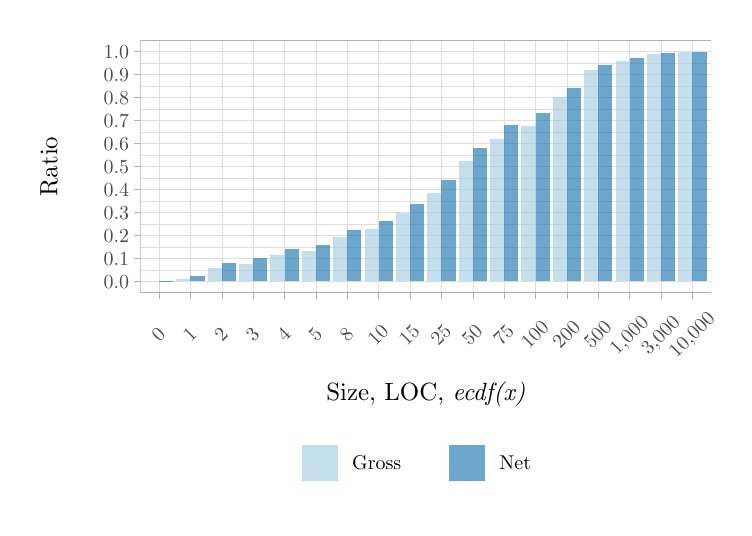
\begin{tikzpicture}[x=1pt,y=1pt]
\definecolor{fillColor}{RGB}{255,255,255}
\path[use as bounding box,fill=fillColor,fill opacity=0.00] (0,0) rectangle (251.50,173.45);
\begin{scope}
\path[clip] (  0.00,  0.00) rectangle (251.50,173.45);
\definecolor{drawColor}{RGB}{255,255,255}
\definecolor{fillColor}{RGB}{255,255,255}

\path[draw=drawColor,line width= 0.5pt,line join=round,line cap=round,fill=fillColor] (  0.00,  0.00) rectangle (251.50,173.45);
\end{scope}
\begin{scope}
\path[clip] ( 40.70, 77.59) rectangle (247.00,168.95);
\definecolor{fillColor}{RGB}{255,255,255}

\path[fill=fillColor] ( 40.70, 77.59) rectangle (247.00,168.95);
\definecolor{drawColor}{gray}{0.87}

\path[draw=drawColor,line width= 0.1pt,line join=round] ( 40.70, 77.59) --
	(247.00, 77.59);

\path[draw=drawColor,line width= 0.1pt,line join=round] ( 40.70, 85.89) --
	(247.00, 85.89);

\path[draw=drawColor,line width= 0.1pt,line join=round] ( 40.70, 94.20) --
	(247.00, 94.20);

\path[draw=drawColor,line width= 0.1pt,line join=round] ( 40.70,102.50) --
	(247.00,102.50);

\path[draw=drawColor,line width= 0.1pt,line join=round] ( 40.70,110.81) --
	(247.00,110.81);

\path[draw=drawColor,line width= 0.1pt,line join=round] ( 40.70,119.11) --
	(247.00,119.11);

\path[draw=drawColor,line width= 0.1pt,line join=round] ( 40.70,127.42) --
	(247.00,127.42);

\path[draw=drawColor,line width= 0.1pt,line join=round] ( 40.70,135.73) --
	(247.00,135.73);

\path[draw=drawColor,line width= 0.1pt,line join=round] ( 40.70,144.03) --
	(247.00,144.03);

\path[draw=drawColor,line width= 0.1pt,line join=round] ( 40.70,152.34) --
	(247.00,152.34);

\path[draw=drawColor,line width= 0.1pt,line join=round] ( 40.70,160.64) --
	(247.00,160.64);

\path[draw=drawColor,line width= 0.1pt,line join=round] ( 40.70,168.95) --
	(247.00,168.95);

\path[draw=drawColor,line width= 0.2pt,line join=round] ( 40.70, 81.74) --
	(247.00, 81.74);

\path[draw=drawColor,line width= 0.2pt,line join=round] ( 40.70, 90.05) --
	(247.00, 90.05);

\path[draw=drawColor,line width= 0.2pt,line join=round] ( 40.70, 98.35) --
	(247.00, 98.35);

\path[draw=drawColor,line width= 0.2pt,line join=round] ( 40.70,106.66) --
	(247.00,106.66);

\path[draw=drawColor,line width= 0.2pt,line join=round] ( 40.70,114.96) --
	(247.00,114.96);

\path[draw=drawColor,line width= 0.2pt,line join=round] ( 40.70,123.27) --
	(247.00,123.27);

\path[draw=drawColor,line width= 0.2pt,line join=round] ( 40.70,131.57) --
	(247.00,131.57);

\path[draw=drawColor,line width= 0.2pt,line join=round] ( 40.70,139.88) --
	(247.00,139.88);

\path[draw=drawColor,line width= 0.2pt,line join=round] ( 40.70,148.18) --
	(247.00,148.18);

\path[draw=drawColor,line width= 0.2pt,line join=round] ( 40.70,156.49) --
	(247.00,156.49);

\path[draw=drawColor,line width= 0.2pt,line join=round] ( 40.70,164.80) --
	(247.00,164.80);

\path[draw=drawColor,line width= 0.2pt,line join=round] ( 47.50, 77.59) --
	( 47.50,168.95);

\path[draw=drawColor,line width= 0.2pt,line join=round] ( 58.83, 77.59) --
	( 58.83,168.95);

\path[draw=drawColor,line width= 0.2pt,line join=round] ( 70.17, 77.59) --
	( 70.17,168.95);

\path[draw=drawColor,line width= 0.2pt,line join=round] ( 81.50, 77.59) --
	( 81.50,168.95);

\path[draw=drawColor,line width= 0.2pt,line join=round] ( 92.84, 77.59) --
	( 92.84,168.95);

\path[draw=drawColor,line width= 0.2pt,line join=round] (104.17, 77.59) --
	(104.17,168.95);

\path[draw=drawColor,line width= 0.2pt,line join=round] (115.51, 77.59) --
	(115.51,168.95);

\path[draw=drawColor,line width= 0.2pt,line join=round] (126.84, 77.59) --
	(126.84,168.95);

\path[draw=drawColor,line width= 0.2pt,line join=round] (138.18, 77.59) --
	(138.18,168.95);

\path[draw=drawColor,line width= 0.2pt,line join=round] (149.52, 77.59) --
	(149.52,168.95);

\path[draw=drawColor,line width= 0.2pt,line join=round] (160.85, 77.59) --
	(160.85,168.95);

\path[draw=drawColor,line width= 0.2pt,line join=round] (172.19, 77.59) --
	(172.19,168.95);

\path[draw=drawColor,line width= 0.2pt,line join=round] (183.52, 77.59) --
	(183.52,168.95);

\path[draw=drawColor,line width= 0.2pt,line join=round] (194.86, 77.59) --
	(194.86,168.95);

\path[draw=drawColor,line width= 0.2pt,line join=round] (206.19, 77.59) --
	(206.19,168.95);

\path[draw=drawColor,line width= 0.2pt,line join=round] (217.53, 77.59) --
	(217.53,168.95);

\path[draw=drawColor,line width= 0.2pt,line join=round] (228.86, 77.59) --
	(228.86,168.95);

\path[draw=drawColor,line width= 0.2pt,line join=round] (240.20, 77.59) --
	(240.20,168.95);
\definecolor{fillColor}{RGB}{31,120,180}

\path[fill=fillColor,fill opacity=0.66] ( 47.50, 81.74) rectangle ( 52.60, 82.03);
\definecolor{fillColor}{RGB}{166,206,227}

\path[fill=fillColor,fill opacity=0.66] ( 42.40, 81.74) rectangle ( 47.50, 81.74);
\definecolor{fillColor}{RGB}{31,120,180}

\path[fill=fillColor,fill opacity=0.66] ( 58.83, 81.74) rectangle ( 63.93, 83.69);
\definecolor{fillColor}{RGB}{166,206,227}

\path[fill=fillColor,fill opacity=0.66] ( 53.73, 81.74) rectangle ( 58.83, 82.53);
\definecolor{fillColor}{RGB}{31,120,180}

\path[fill=fillColor,fill opacity=0.66] ( 70.17, 81.74) rectangle ( 75.27, 88.25);
\definecolor{fillColor}{RGB}{166,206,227}

\path[fill=fillColor,fill opacity=0.66] ( 65.07, 81.74) rectangle ( 70.17, 86.73);
\definecolor{fillColor}{RGB}{31,120,180}

\path[fill=fillColor,fill opacity=0.66] ( 81.50, 81.74) rectangle ( 86.60, 90.27);
\definecolor{fillColor}{RGB}{166,206,227}

\path[fill=fillColor,fill opacity=0.66] ( 76.40, 81.74) rectangle ( 81.50, 88.10);
\definecolor{fillColor}{RGB}{31,120,180}

\path[fill=fillColor,fill opacity=0.66] ( 92.84, 81.74) rectangle ( 97.94, 93.45);
\definecolor{fillColor}{RGB}{166,206,227}

\path[fill=fillColor,fill opacity=0.66] ( 87.74, 81.74) rectangle ( 92.84, 91.14);
\definecolor{fillColor}{RGB}{31,120,180}

\path[fill=fillColor,fill opacity=0.66] (104.17, 81.74) rectangle (109.27, 94.75);
\definecolor{fillColor}{RGB}{166,206,227}

\path[fill=fillColor,fill opacity=0.66] ( 99.07, 81.74) rectangle (104.17, 92.73);
\definecolor{fillColor}{RGB}{31,120,180}

\path[fill=fillColor,fill opacity=0.66] (115.51, 81.74) rectangle (120.61,100.17);
\definecolor{fillColor}{RGB}{166,206,227}

\path[fill=fillColor,fill opacity=0.66] (110.41, 81.74) rectangle (115.51, 97.64);
\definecolor{fillColor}{RGB}{31,120,180}

\path[fill=fillColor,fill opacity=0.66] (126.84, 81.74) rectangle (131.95,103.71);
\definecolor{fillColor}{RGB}{166,206,227}

\path[fill=fillColor,fill opacity=0.66] (121.74, 81.74) rectangle (126.84,100.61);
\definecolor{fillColor}{RGB}{31,120,180}

\path[fill=fillColor,fill opacity=0.66] (138.18, 81.74) rectangle (143.28,109.64);
\definecolor{fillColor}{RGB}{166,206,227}

\path[fill=fillColor,fill opacity=0.66] (133.08, 81.74) rectangle (138.18,106.39);
\definecolor{fillColor}{RGB}{31,120,180}

\path[fill=fillColor,fill opacity=0.66] (149.52, 81.74) rectangle (154.62,118.32);
\definecolor{fillColor}{RGB}{166,206,227}

\path[fill=fillColor,fill opacity=0.66] (144.41, 81.74) rectangle (149.52,113.69);
\definecolor{fillColor}{RGB}{31,120,180}

\path[fill=fillColor,fill opacity=0.66] (160.85, 81.74) rectangle (165.95,130.10);
\definecolor{fillColor}{RGB}{166,206,227}

\path[fill=fillColor,fill opacity=0.66] (155.75, 81.74) rectangle (160.85,125.40);
\definecolor{fillColor}{RGB}{31,120,180}

\path[fill=fillColor,fill opacity=0.66] (172.19, 81.74) rectangle (177.29,138.12);
\definecolor{fillColor}{RGB}{166,206,227}

\path[fill=fillColor,fill opacity=0.66] (167.09, 81.74) rectangle (172.19,133.13);
\definecolor{fillColor}{RGB}{31,120,180}

\path[fill=fillColor,fill opacity=0.66] (183.52, 81.74) rectangle (188.62,142.46);
\definecolor{fillColor}{RGB}{166,206,227}

\path[fill=fillColor,fill opacity=0.66] (178.42, 81.74) rectangle (183.52,137.91);
\definecolor{fillColor}{RGB}{31,120,180}

\path[fill=fillColor,fill opacity=0.66] (194.86, 81.74) rectangle (199.96,151.71);
\definecolor{fillColor}{RGB}{166,206,227}

\path[fill=fillColor,fill opacity=0.66] (189.76, 81.74) rectangle (194.86,148.31);
\definecolor{fillColor}{RGB}{31,120,180}

\path[fill=fillColor,fill opacity=0.66] (206.19, 81.74) rectangle (211.29,159.88);
\definecolor{fillColor}{RGB}{166,206,227}

\path[fill=fillColor,fill opacity=0.66] (201.09, 81.74) rectangle (206.19,158.14);
\definecolor{fillColor}{RGB}{31,120,180}

\path[fill=fillColor,fill opacity=0.66] (217.53, 81.74) rectangle (222.63,162.63);
\definecolor{fillColor}{RGB}{166,206,227}

\path[fill=fillColor,fill opacity=0.66] (212.43, 81.74) rectangle (217.53,161.54);
\definecolor{fillColor}{RGB}{31,120,180}

\path[fill=fillColor,fill opacity=0.66] (228.86, 81.74) rectangle (233.96,164.43);
\definecolor{fillColor}{RGB}{166,206,227}

\path[fill=fillColor,fill opacity=0.66] (223.76, 81.74) rectangle (228.86,163.93);
\definecolor{fillColor}{RGB}{31,120,180}

\path[fill=fillColor,fill opacity=0.66] (240.20, 81.74) rectangle (245.30,164.72);
\definecolor{fillColor}{RGB}{166,206,227}

\path[fill=fillColor,fill opacity=0.66] (235.10, 81.74) rectangle (240.20,164.65);
\definecolor{drawColor}{gray}{0.70}

\path[draw=drawColor,line width= 0.5pt,line join=round,line cap=round] ( 40.70, 77.59) rectangle (247.00,168.95);
\end{scope}
\begin{scope}
\path[clip] (  0.00,  0.00) rectangle (251.50,173.45);
\definecolor{drawColor}{gray}{0.30}

\node[text=drawColor,anchor=base east,inner sep=0pt, outer sep=0pt, scale=  0.72] at ( 36.65, 79.26) {0.0};

\node[text=drawColor,anchor=base east,inner sep=0pt, outer sep=0pt, scale=  0.72] at ( 36.65, 87.57) {0.1};

\node[text=drawColor,anchor=base east,inner sep=0pt, outer sep=0pt, scale=  0.72] at ( 36.65, 95.87) {0.2};

\node[text=drawColor,anchor=base east,inner sep=0pt, outer sep=0pt, scale=  0.72] at ( 36.65,104.18) {0.3};

\node[text=drawColor,anchor=base east,inner sep=0pt, outer sep=0pt, scale=  0.72] at ( 36.65,112.48) {0.4};

\node[text=drawColor,anchor=base east,inner sep=0pt, outer sep=0pt, scale=  0.72] at ( 36.65,120.79) {0.5};

\node[text=drawColor,anchor=base east,inner sep=0pt, outer sep=0pt, scale=  0.72] at ( 36.65,129.09) {0.6};

\node[text=drawColor,anchor=base east,inner sep=0pt, outer sep=0pt, scale=  0.72] at ( 36.65,137.40) {0.7};

\node[text=drawColor,anchor=base east,inner sep=0pt, outer sep=0pt, scale=  0.72] at ( 36.65,145.70) {0.8};

\node[text=drawColor,anchor=base east,inner sep=0pt, outer sep=0pt, scale=  0.72] at ( 36.65,154.01) {0.9};

\node[text=drawColor,anchor=base east,inner sep=0pt, outer sep=0pt, scale=  0.72] at ( 36.65,162.32) {1.0};
\end{scope}
\begin{scope}
\path[clip] (  0.00,  0.00) rectangle (251.50,173.45);
\definecolor{drawColor}{gray}{0.70}

\path[draw=drawColor,line width= 0.2pt,line join=round] ( 38.45, 81.74) --
	( 40.70, 81.74);

\path[draw=drawColor,line width= 0.2pt,line join=round] ( 38.45, 90.05) --
	( 40.70, 90.05);

\path[draw=drawColor,line width= 0.2pt,line join=round] ( 38.45, 98.35) --
	( 40.70, 98.35);

\path[draw=drawColor,line width= 0.2pt,line join=round] ( 38.45,106.66) --
	( 40.70,106.66);

\path[draw=drawColor,line width= 0.2pt,line join=round] ( 38.45,114.96) --
	( 40.70,114.96);

\path[draw=drawColor,line width= 0.2pt,line join=round] ( 38.45,123.27) --
	( 40.70,123.27);

\path[draw=drawColor,line width= 0.2pt,line join=round] ( 38.45,131.57) --
	( 40.70,131.57);

\path[draw=drawColor,line width= 0.2pt,line join=round] ( 38.45,139.88) --
	( 40.70,139.88);

\path[draw=drawColor,line width= 0.2pt,line join=round] ( 38.45,148.18) --
	( 40.70,148.18);

\path[draw=drawColor,line width= 0.2pt,line join=round] ( 38.45,156.49) --
	( 40.70,156.49);

\path[draw=drawColor,line width= 0.2pt,line join=round] ( 38.45,164.80) --
	( 40.70,164.80);
\end{scope}
\begin{scope}
\path[clip] (  0.00,  0.00) rectangle (251.50,173.45);
\definecolor{drawColor}{gray}{0.70}

\path[draw=drawColor,line width= 0.2pt,line join=round] ( 47.50, 75.34) --
	( 47.50, 77.59);

\path[draw=drawColor,line width= 0.2pt,line join=round] ( 58.83, 75.34) --
	( 58.83, 77.59);

\path[draw=drawColor,line width= 0.2pt,line join=round] ( 70.17, 75.34) --
	( 70.17, 77.59);

\path[draw=drawColor,line width= 0.2pt,line join=round] ( 81.50, 75.34) --
	( 81.50, 77.59);

\path[draw=drawColor,line width= 0.2pt,line join=round] ( 92.84, 75.34) --
	( 92.84, 77.59);

\path[draw=drawColor,line width= 0.2pt,line join=round] (104.17, 75.34) --
	(104.17, 77.59);

\path[draw=drawColor,line width= 0.2pt,line join=round] (115.51, 75.34) --
	(115.51, 77.59);

\path[draw=drawColor,line width= 0.2pt,line join=round] (126.84, 75.34) --
	(126.84, 77.59);

\path[draw=drawColor,line width= 0.2pt,line join=round] (138.18, 75.34) --
	(138.18, 77.59);

\path[draw=drawColor,line width= 0.2pt,line join=round] (149.52, 75.34) --
	(149.52, 77.59);

\path[draw=drawColor,line width= 0.2pt,line join=round] (160.85, 75.34) --
	(160.85, 77.59);

\path[draw=drawColor,line width= 0.2pt,line join=round] (172.19, 75.34) --
	(172.19, 77.59);

\path[draw=drawColor,line width= 0.2pt,line join=round] (183.52, 75.34) --
	(183.52, 77.59);

\path[draw=drawColor,line width= 0.2pt,line join=round] (194.86, 75.34) --
	(194.86, 77.59);

\path[draw=drawColor,line width= 0.2pt,line join=round] (206.19, 75.34) --
	(206.19, 77.59);

\path[draw=drawColor,line width= 0.2pt,line join=round] (217.53, 75.34) --
	(217.53, 77.59);

\path[draw=drawColor,line width= 0.2pt,line join=round] (228.86, 75.34) --
	(228.86, 77.59);

\path[draw=drawColor,line width= 0.2pt,line join=round] (240.20, 75.34) --
	(240.20, 77.59);
\end{scope}
\begin{scope}
\path[clip] (  0.00,  0.00) rectangle (251.50,173.45);
\definecolor{drawColor}{gray}{0.30}

\node[text=drawColor,rotate= 45.00,anchor=base,inner sep=0pt, outer sep=0pt, scale=  0.72] at ( 48.90, 60.95) {     0};

\node[text=drawColor,rotate= 45.00,anchor=base,inner sep=0pt, outer sep=0pt, scale=  0.72] at ( 60.23, 60.95) {     1};

\node[text=drawColor,rotate= 45.00,anchor=base,inner sep=0pt, outer sep=0pt, scale=  0.72] at ( 71.57, 60.95) {     2};

\node[text=drawColor,rotate= 45.00,anchor=base,inner sep=0pt, outer sep=0pt, scale=  0.72] at ( 82.91, 60.95) {     3};

\node[text=drawColor,rotate= 45.00,anchor=base,inner sep=0pt, outer sep=0pt, scale=  0.72] at ( 94.24, 60.95) {     4};

\node[text=drawColor,rotate= 45.00,anchor=base,inner sep=0pt, outer sep=0pt, scale=  0.72] at (105.58, 60.95) {     5};

\node[text=drawColor,rotate= 45.00,anchor=base,inner sep=0pt, outer sep=0pt, scale=  0.72] at (116.91, 60.95) {     8};

\node[text=drawColor,rotate= 45.00,anchor=base,inner sep=0pt, outer sep=0pt, scale=  0.72] at (128.25, 60.95) {    10};

\node[text=drawColor,rotate= 45.00,anchor=base,inner sep=0pt, outer sep=0pt, scale=  0.72] at (139.58, 60.95) {    15};

\node[text=drawColor,rotate= 45.00,anchor=base,inner sep=0pt, outer sep=0pt, scale=  0.72] at (150.92, 60.95) {    25};

\node[text=drawColor,rotate= 45.00,anchor=base,inner sep=0pt, outer sep=0pt, scale=  0.72] at (162.25, 60.95) {    50};

\node[text=drawColor,rotate= 45.00,anchor=base,inner sep=0pt, outer sep=0pt, scale=  0.72] at (173.59, 60.95) {    75};

\node[text=drawColor,rotate= 45.00,anchor=base,inner sep=0pt, outer sep=0pt, scale=  0.72] at (184.92, 60.95) {   100};

\node[text=drawColor,rotate= 45.00,anchor=base,inner sep=0pt, outer sep=0pt, scale=  0.72] at (196.26, 60.95) {   200};

\node[text=drawColor,rotate= 45.00,anchor=base,inner sep=0pt, outer sep=0pt, scale=  0.72] at (207.59, 60.95) {   500};

\node[text=drawColor,rotate= 45.00,anchor=base,inner sep=0pt, outer sep=0pt, scale=  0.72] at (218.93, 60.95) { 1,000};

\node[text=drawColor,rotate= 45.00,anchor=base,inner sep=0pt, outer sep=0pt, scale=  0.72] at (230.27, 60.95) { 3,000};

\node[text=drawColor,rotate= 45.00,anchor=base,inner sep=0pt, outer sep=0pt, scale=  0.72] at (241.60, 60.95) {10,000};
\end{scope}
\begin{scope}
\path[clip] (  0.00,  0.00) rectangle (251.50,173.45);
\definecolor{drawColor}{RGB}{0,0,0}

\node[text=drawColor,anchor=base,inner sep=0pt, outer sep=0pt, scale=  0.90] at (143.85, 38.70) {Size, LOC, $\textit{ecdf(x)}$};
\end{scope}
\begin{scope}
\path[clip] (  0.00,  0.00) rectangle (251.50,173.45);
\definecolor{drawColor}{RGB}{0,0,0}

\node[text=drawColor,rotate= 90.00,anchor=base,inner sep=0pt, outer sep=0pt, scale=  0.90] at ( 10.70,123.27) {Ratio};
\end{scope}
\begin{scope}
\path[clip] (  0.00,  0.00) rectangle (251.50,173.45);
\definecolor{fillColor}{RGB}{255,255,255}

\path[fill=fillColor] ( 89.32,  4.50) rectangle (198.37, 27.95);
\end{scope}
\begin{scope}
\path[clip] (  0.00,  0.00) rectangle (251.50,173.45);
\definecolor{fillColor}{RGB}{255,255,255}

\path[fill=fillColor] ( 98.32,  9.00) rectangle (112.78, 23.45);
\end{scope}
\begin{scope}
\path[clip] (  0.00,  0.00) rectangle (251.50,173.45);
\definecolor{fillColor}{RGB}{166,206,227}

\path[fill=fillColor,fill opacity=0.66] ( 99.03,  9.71) rectangle (112.06, 22.74);
\end{scope}
\begin{scope}
\path[clip] (  0.00,  0.00) rectangle (251.50,173.45);
\definecolor{fillColor}{RGB}{255,255,255}

\path[fill=fillColor] (151.52,  9.00) rectangle (165.98, 23.45);
\end{scope}
\begin{scope}
\path[clip] (  0.00,  0.00) rectangle (251.50,173.45);
\definecolor{fillColor}{RGB}{31,120,180}

\path[fill=fillColor,fill opacity=0.66] (152.23,  9.71) rectangle (165.26, 22.74);
\end{scope}
\begin{scope}
\path[clip] (  0.00,  0.00) rectangle (251.50,173.45);
\definecolor{drawColor}{RGB}{0,0,0}

\node[text=drawColor,anchor=base west,inner sep=0pt, outer sep=0pt, scale=  0.72] at (117.28, 13.75) {Gross};
\end{scope}
\begin{scope}
\path[clip] (  0.00,  0.00) rectangle (251.50,173.45);
\definecolor{drawColor}{RGB}{0,0,0}

\node[text=drawColor,anchor=base west,inner sep=0pt, outer sep=0pt, scale=  0.72] at (170.48, 13.75) {Net};
\end{scope}
\end{tikzpicture}
